En último lugar realizaremos un estudio de la linealidad del PMT. 

En primer lugar buscamos testear esta linealidad al orden de número de fotones de un evento del agua tritiada ya que este será su objetivo final. Si tenemos en cuenta que, según el espectro de desintegración del tritio, sus eventos poseen una energía promedio de $5.7~\keV$ y que las fibras, según Saint-Gobain, poseen una eficiencia de fluorescencia de $8000~\gamma/\MeV$ para un mip (valor que se pretende comprobar en un futuro inmediato), podemos observar que un evento promedio del tritió corresponderá a $45$ fotones aproximadamente. Si tenemos en cuenta además la existencia de una lijera pérdida debido a la no existencia del clad en la fibra vemos que, este evento corresponderá a unas pocas decenas de fotones.

Para comprobar la linealidad del PMT a eventos de este orden utilizamos el dispositivo mostrado en la figura \ref{esquemasetup} donde situaremos el PMT a $200~\mm$ del diodo LED. Además, en este estudio no utilizaremos ninguna fibra y trabajaremos en el rango de linealidad del LED (alimentación hasta un máximo 5 amperios), de esta forma podemos asegurar que, en caso de producirse una no linealidad, esta será debida únicamente a la saturación del PMT. 

También utilizaremos colimadores para asegurar que la superficie activa con la que estamos leyendo es la del diametro de la fibra ya que, aunque un evento que no produzca saturación del PMT puede que, al reducir su superficie activa de detección, un evento de la misma energía si produzca saturación.

El resultado de este primer experimento se muestra en la figura \ref{linealidadordentritio}

\begin{figure}[H]
\centering
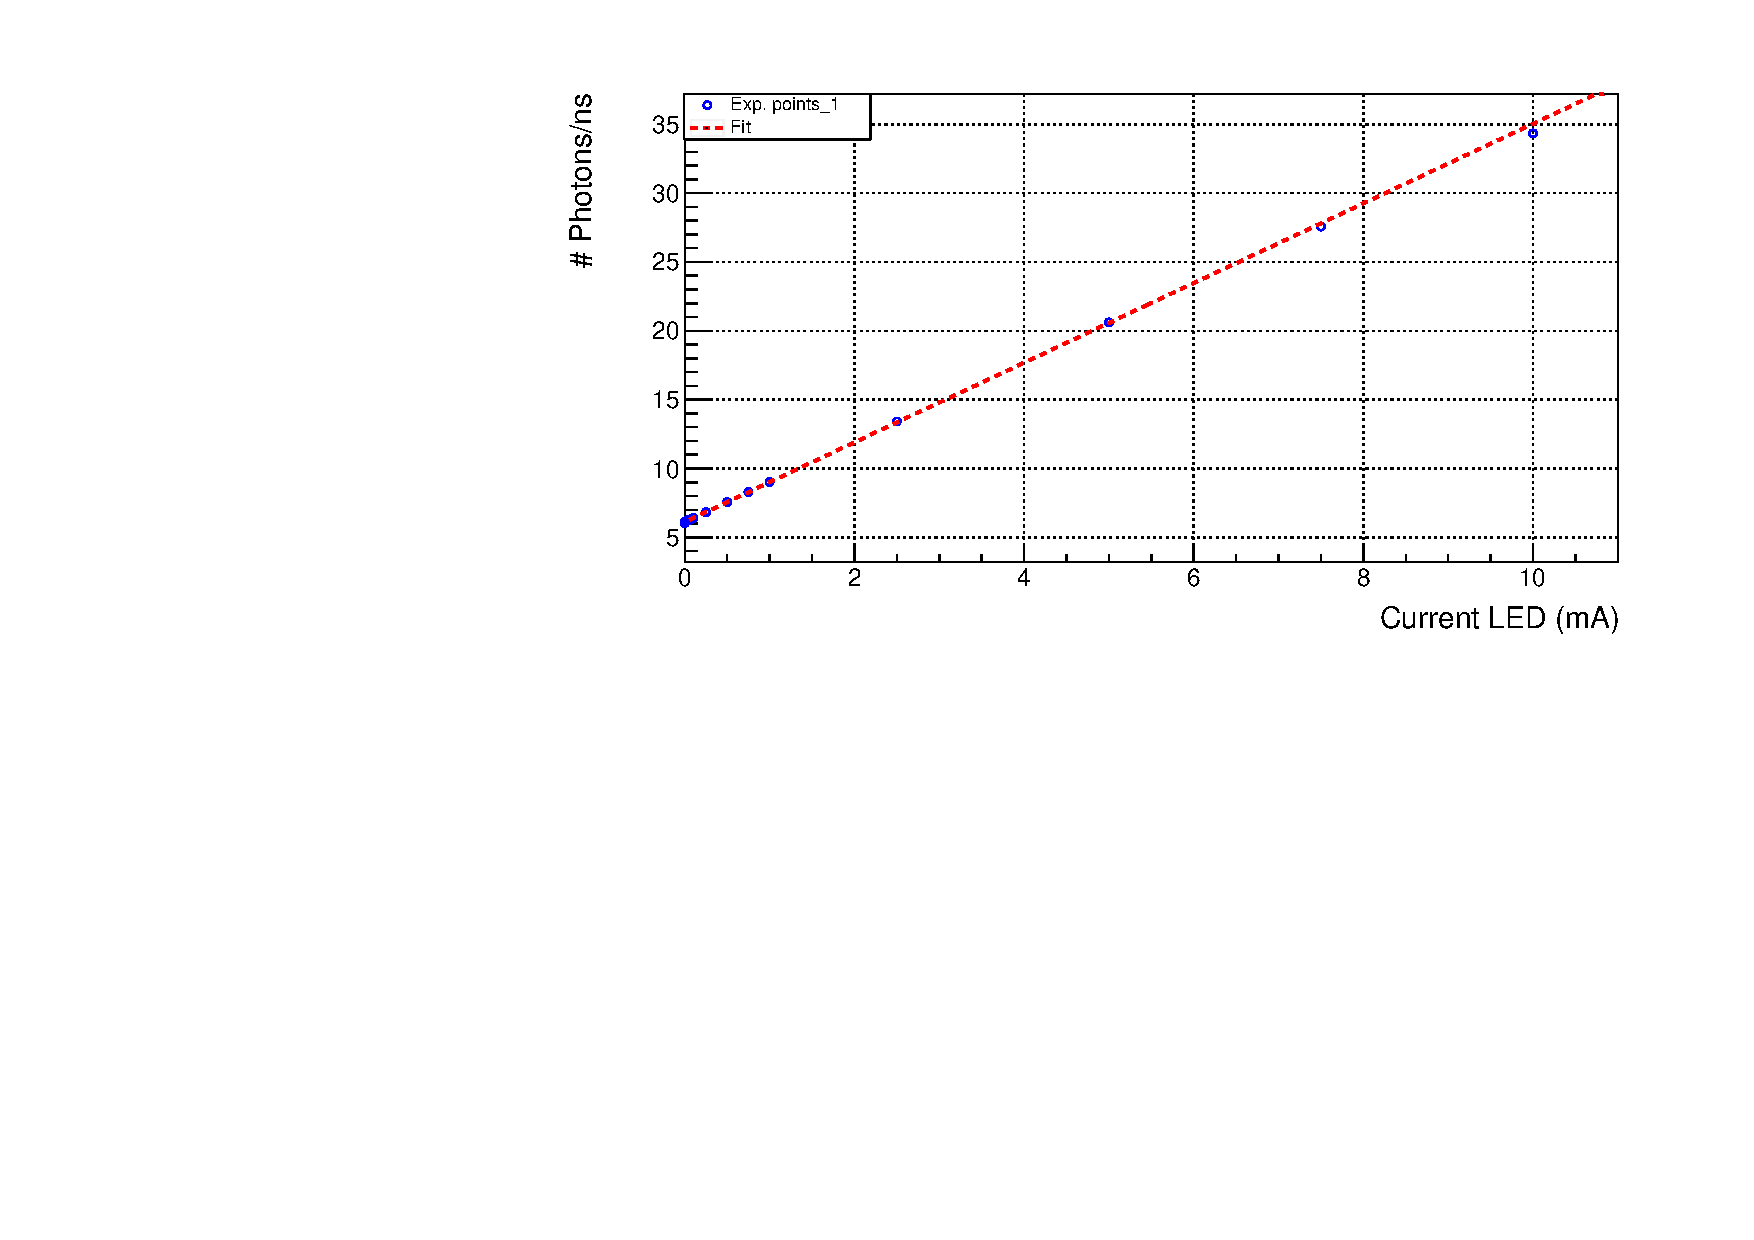
\includegraphics[scale=0.7]{Figuras/fit1background.pdf}
\caption{Respuesta del PMT utilizado en el experimento\label{linealidadordentritio}}
\end{figure}

Con esta gráfica podemos observar que, efectivamente, en el caso de que la actividad de la disolución de agua tritiada que pretendemos medir sea lo suficientemente baja para que el PMT no tenga pile-up este se comportará de forma perfectamente lineal, lo cual es fundamental si queremos realizar la monitorización de la actividad del tritio.

En la figura \ref{linealidadordentritio} puedo observarse que para intensidades de alimentación de la led muy bajas (inferior a $0.5~\milli\ampere$) se tomó un paso mucho menor. La figura \ref{zoomtransicion} muestra una ampliación de la región entre $0$ y $0.22~\milli\ampere$ y la figura \ref{zoomtransicion2} muestra una ampliación todavía mayor de la región entre $0$ y $0.005~\milli\ampere$.

\begin{figure}[H]
\centering
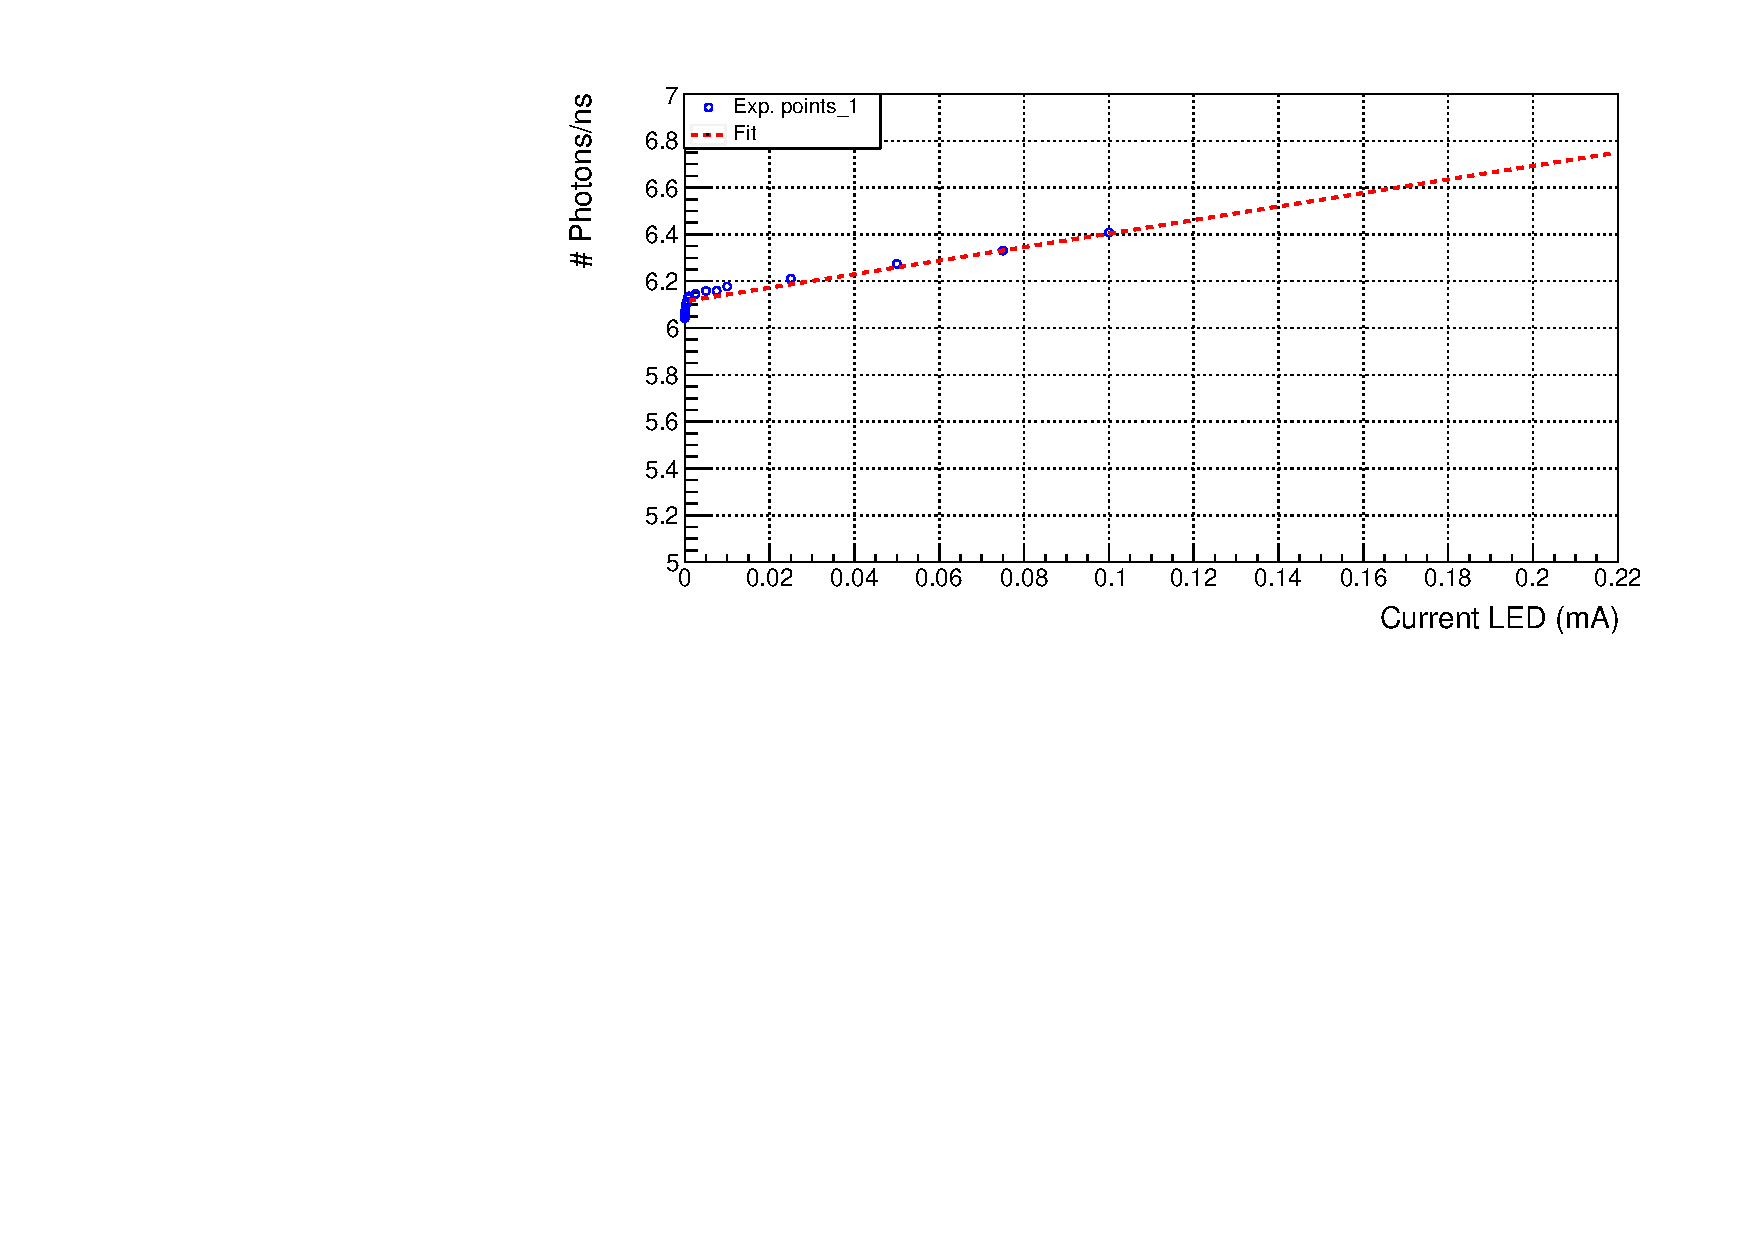
\includegraphics[scale=0.7]{Figuras/Transicionbackground.pdf}
\caption{Ampliación de la zona de transición\label{zoomtransicion}}
\end{figure}

\begin{figure}[H]
\centering
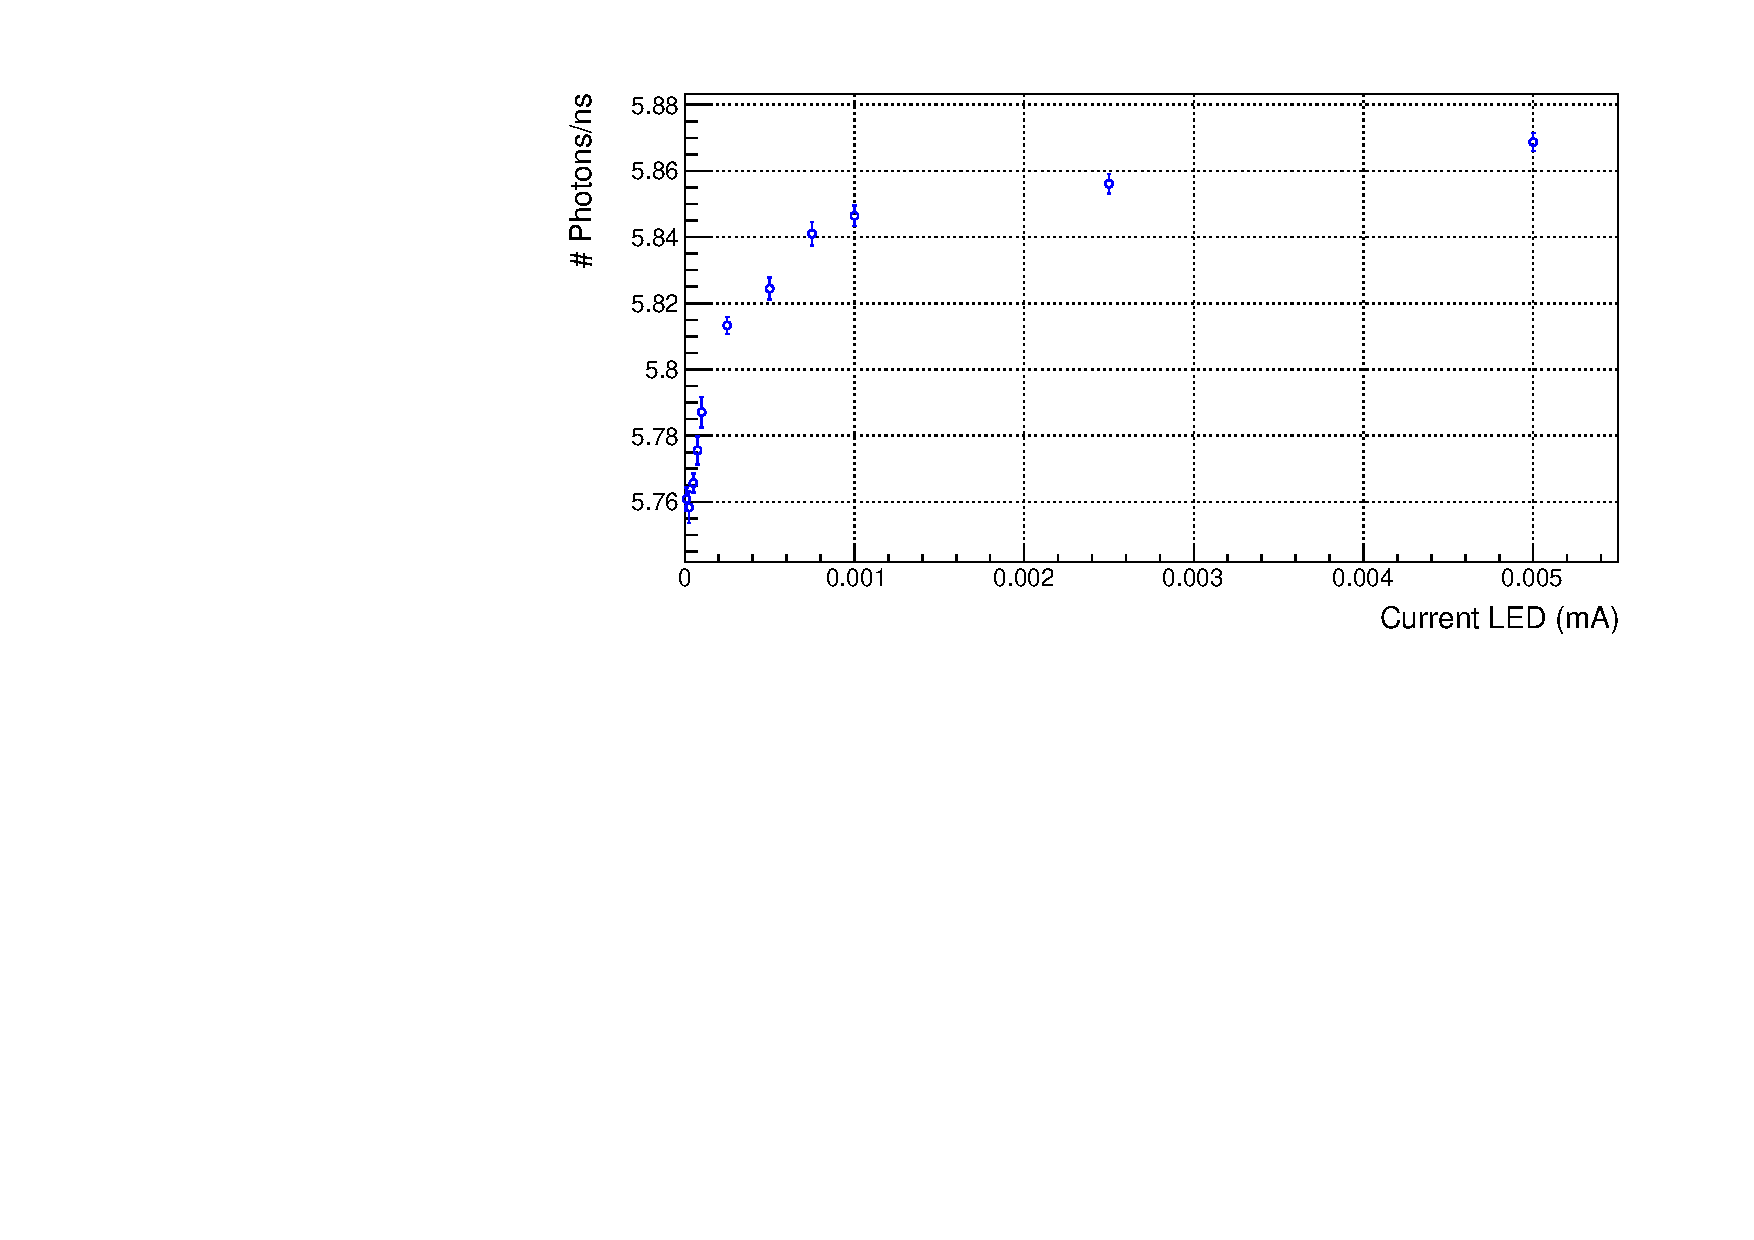
\includegraphics[scale=0.7]{Figuras/Transicionbackground2.pdf}
\caption{Ampliación de la zona de transición\label{zoomtransicion2}}
\end{figure}

Podemos observar que la existencia de una no linealidad en el comportamiento de nuestro sistema. Esto es debido al comportamiento de la LED cuya relación característia es:

\begin{equation}
I=I_s(e^{V_D/{nV_T}}-1)
\label{LED}
\end{equation}

Donde lo único que nos importa de esta expresión es que la dependencia entre la intensidad emitida por la led $I$ (número de fotones por unidad de tiempo) y el voltaje con el que esta se alimenta $V_D$ (el cual es proporcional a la intensidad con la que estamos alimentando) es una exponencial. Esta expresión, en primer orden de magnitud, puede aproximarse a una dependencia lineal. Este es el origen de la dependencia lineal entre la intensidad emitida por la LED y la intensidad con la que la alimentamos. Sin embargo, hay que tener en cuenta que el diodo LED consta de una unión PN de dos materiales semiconductores. Por ello, necesita alimentar con un voltaje mínimo (usualmente $V_{min}\approx 0.7~\volt$ para LEDs comerciales) a partir del cual los portadores de carga (electrones) tienen suficiente energía para pasar a la región de conducción. Es por ello que el diodo LED necesita un voltaje de alimentación mínimo (o, en nuestro caso, una intensidad de alimentación  mínima) para emitir fotones.

Realmente esta transición no es importante desde el punto de vista del proyecto tritium ya que este no utiliza el diodo LED. En el detector la fuente de fotones serán los diversos eventos de tritio capturados por las fibras. Además hemos visto que estos eventos tendrán del orden de unas pocas decenas de fotones donde, anteriormente, hemos comprobado que el sistema es lineal. 

Sin embargo es importante documentar esta púnto de mínima intensidad de alimentación de la LED ya que, para asegurar el correcto funcionamiento del sistema, debemos situarnos por encima de este punto, el cual, en la figura \ref{zoomtransicion2}, podemos ver que es $0.001~\milli\ampere$.

Finalmente, por completitud, extendemos el rango en dos ocasiones. En primer lugar lo extendemos hasta un máximo de $300~\gamma/\nano\second$, el cual puede verse en la figura \ref{300} y, en segundo lugar, lo extendemos hasta un máximo de $2500~\gamma/\nano\second$, el cual puede verse en la figura \ref{2500}

\begin{figure}[H]
\centering
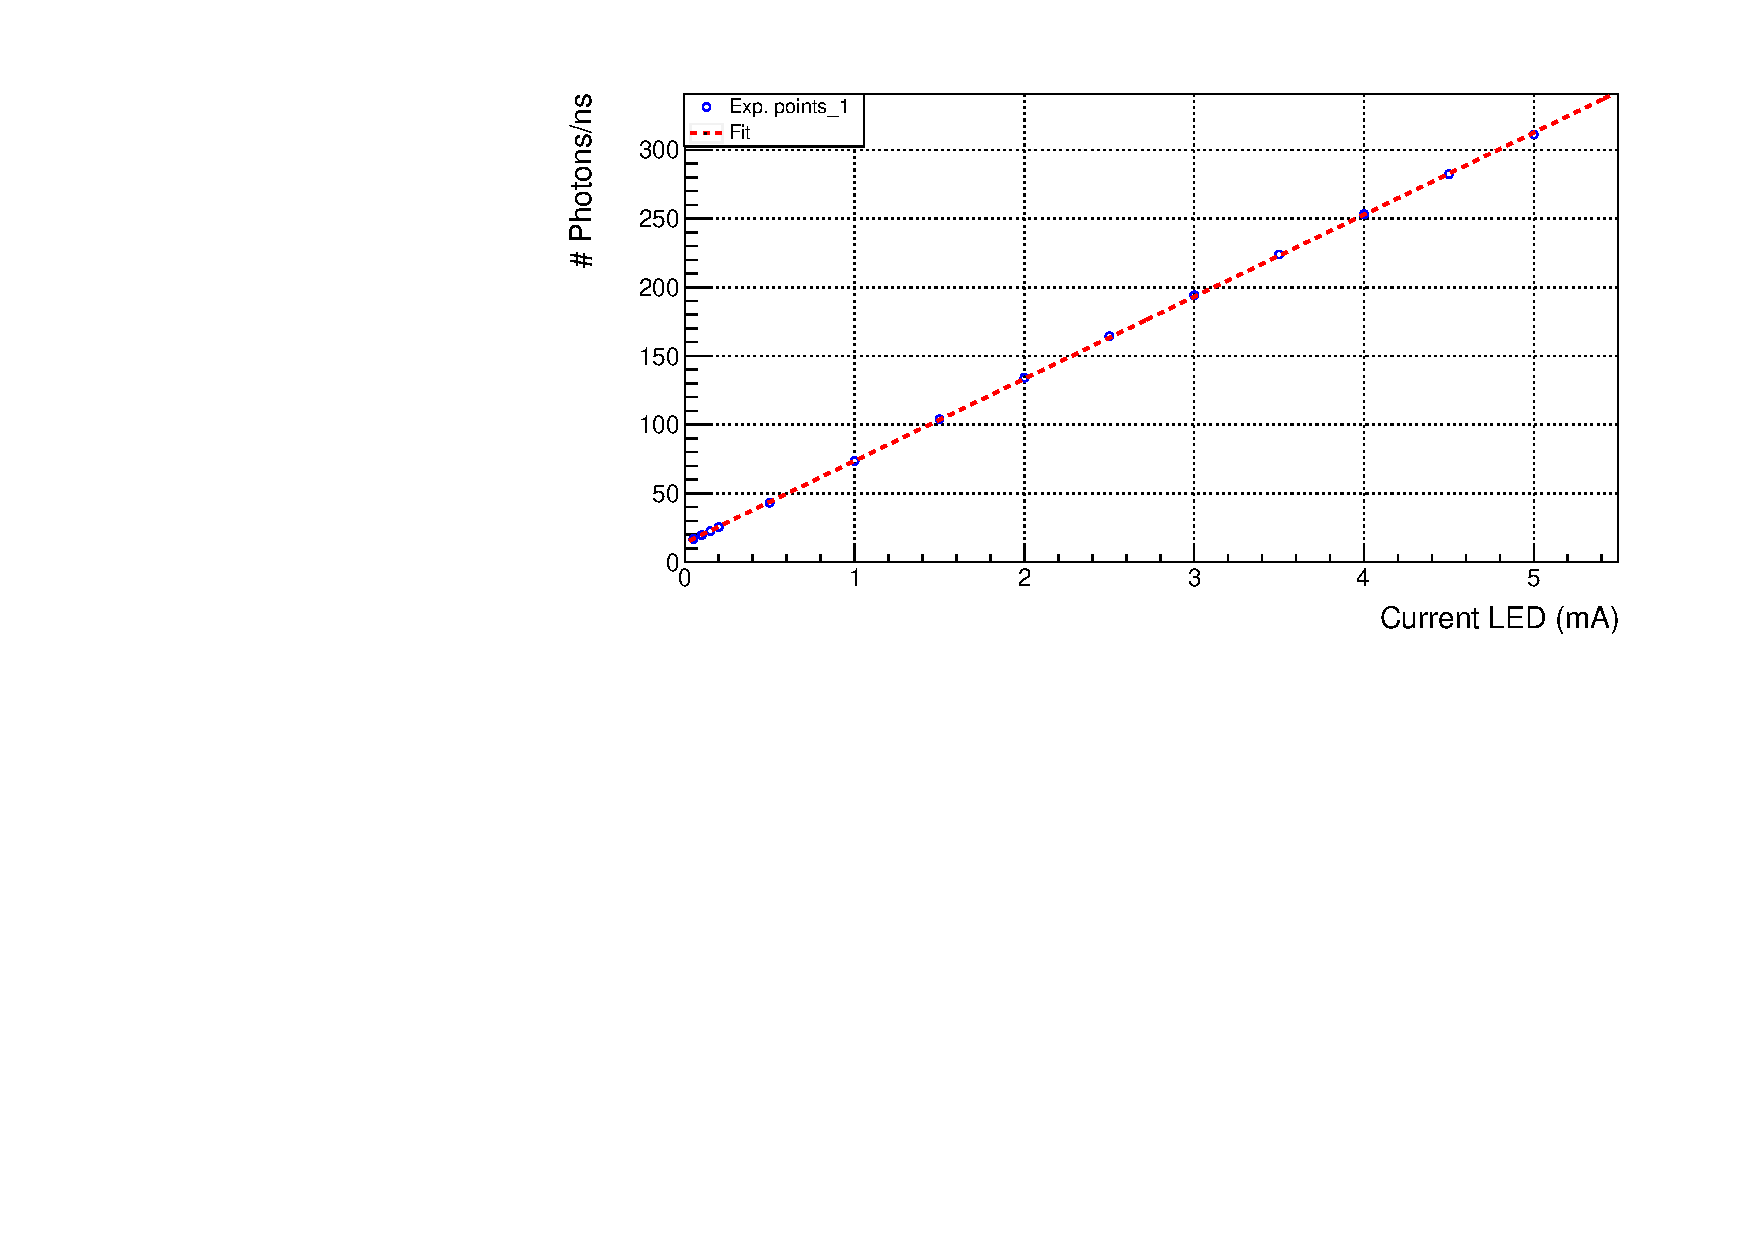
\includegraphics[scale=0.7]{Figuras/300.pdf}
\caption{Ampliación del intervalo de respuesta estudiado hasta 300 fotones por nanosegundo\label{300}}
\end{figure}

\begin{figure}[H]
\centering
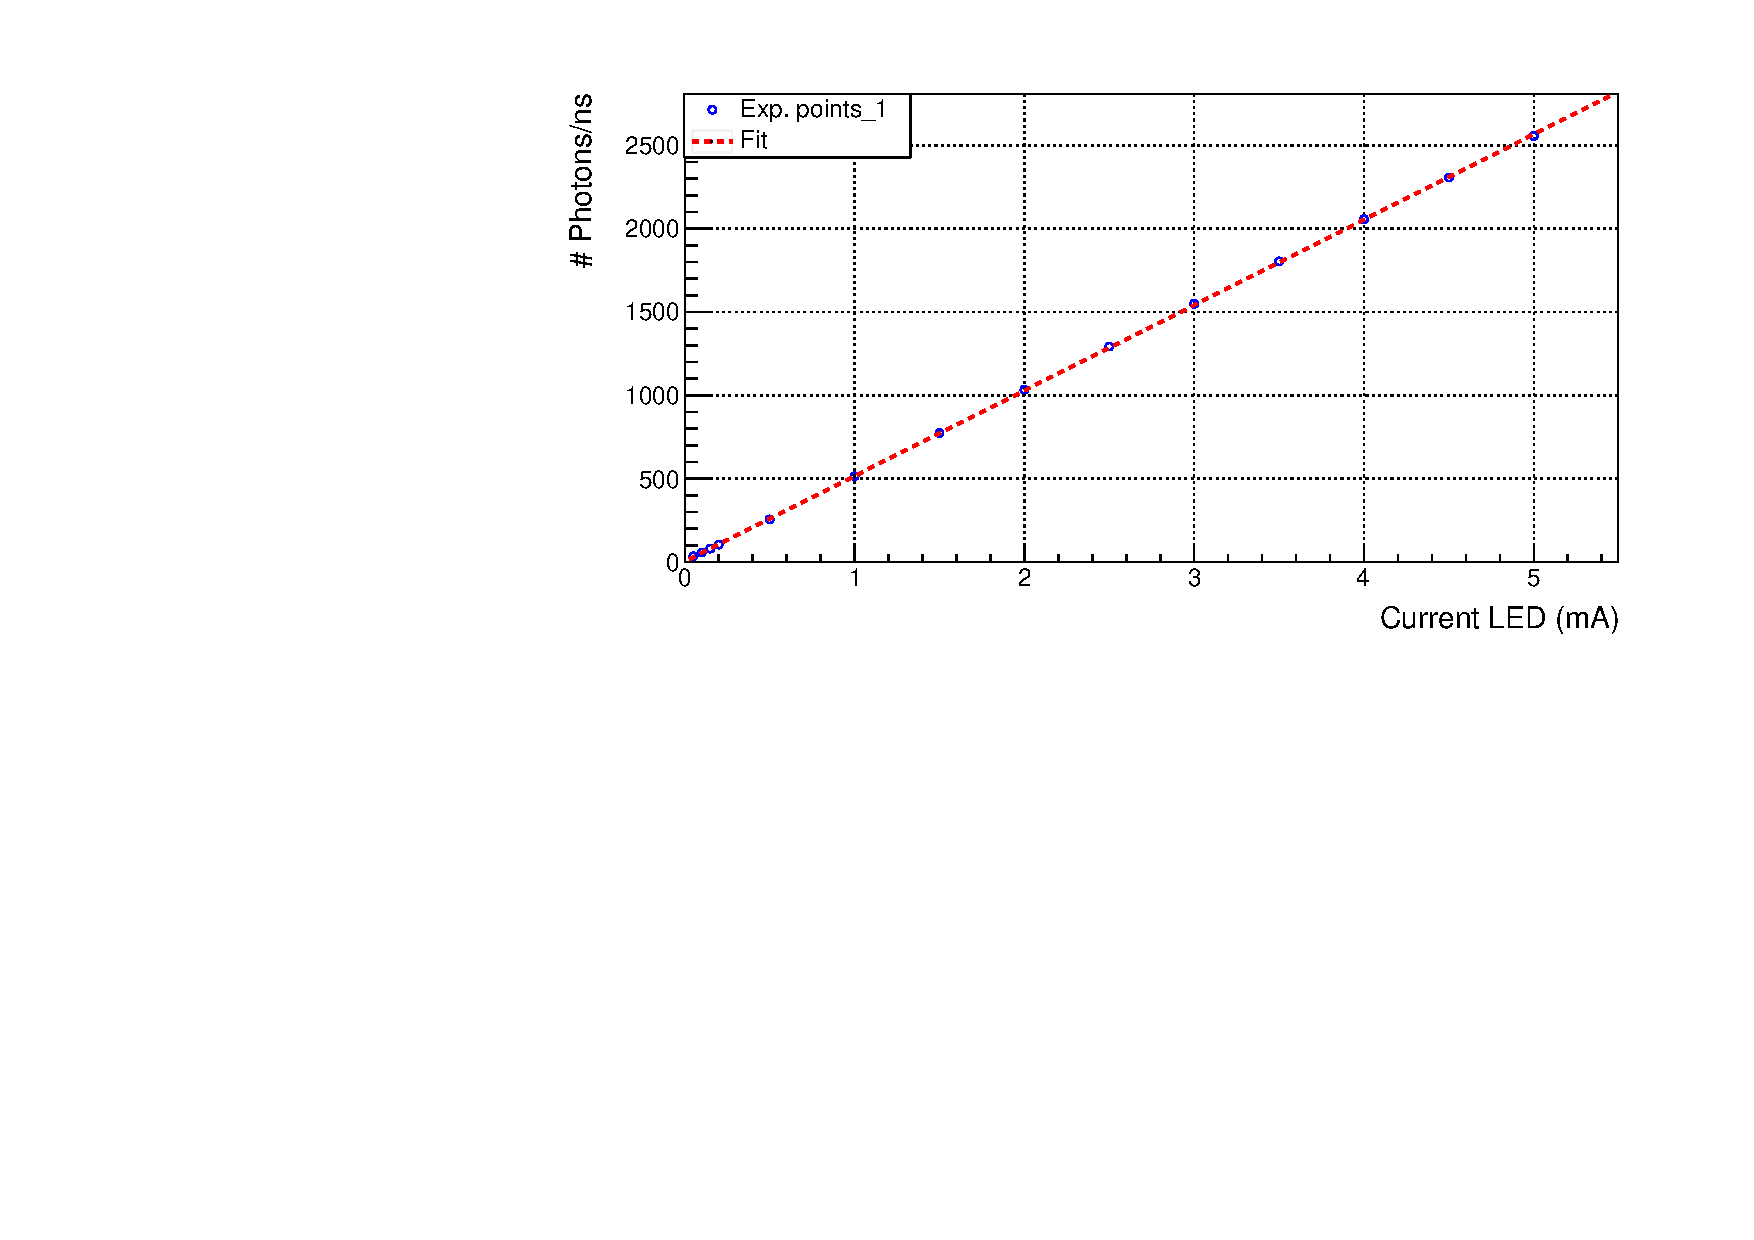
\includegraphics[scale=0.7]{Figuras/2500.pdf}
\caption{Ampliación del intervalo de respuesta estudiado hasta 2500 fotones por nanosegundo\label{2500}}
\end{figure}

En ambos espectros podemos observar que el comportamiento del sistema es perfectamente lineal. Por tanto, en resumen, hemos comprobado que, si alimentamos con más de $0.001~\milli\ampere$ la LED, el sistema es perfectamente lineal hasta $2500~\gamma/\nano\second$ a partir del cual ya no extenderemos más nuestro estudio de linealidad porque no tendremos señales mayores. 